\documentclass[12pt]{article}
%\usepackage{eacl2014}
%\usepackage{times}
\usepackage{apacite}
\usepackage{url}
\usepackage{latexsym}
\usepackage{covington}
\usepackage{graphicx}
\usepackage{float}
\usepackage{qtree}
\usepackage{setspace}
\doublespacing

%\special{papersize=210mm,297mm} % to avoid having to use "-t a4" with dvips 
%\setlength \titlebox{6.5cm}  % You can expand the title box if you really have to

\title{Improving word prediction for augmentative communication by using idiolects and sociolects}

\author{
Wessel Stoop\vspace{-2ex}\\
Centre for Language and Speech Technology\vspace{-2ex}\\
Radboud University Nijmegen\vspace{-2ex} \\
  {\tt w.stoop@let.ru.nl} \\
  \and
  Antal van den Bosch \vspace{-2ex}\\
Centre for Language Studies \vspace{-2ex}\\
Radboud University Nijmegen \vspace{-2ex}\\
  {\tt a.vandenbosch@let.ru.nl} \vspace{-2ex}\\
}

\date{}

%Set font
%\renewcommand{\familydefault}{\sfdefault}

%Tables captions small
%\usepackage{caption3} % load caption package kernel first
%\DeclareCaptionOption{parskip}[]{} % disable "parskip" caption option
%\usepackage[footnotesize]{caption}

%Line spacing
%\linespread{1.5}

%New page for every chapter
%\let\stdsection\section
%\renewcommand\section{\newpage\stdsection}

%Center tables
\let\originaltable\table
\let\endoriginaltable\endtable
\renewenvironment{table}[1][ht]{%
  \originaltable[#1]
  \centering}%
  {\endoriginaltable}

\begin{document}

\maketitle

\begin{abstract}
Word prediction, or predictive editing, now a commodity technology on mobile devices, has a long history as a tool for augmentative and assistive communication. The state-of-the-art has been pushed forward, but major improvements can still be achieved, for instance by training personalized statistical language models.
To explore this challenge we developed the word prediction system \emph{Soothsayer}
\footnote{Name of the system has been anonymized. The system is available as an interactive demo at \url{http://soothsayer.cls.ru.nl/} and its source code is publicly available at \url{https://https://github.com/Woseseltops/soothsayer}}. 

This system predicts what a user is going to write as he is keying it in. The main innovation of Soothsayer is that it not only uses \emph{idiolects}, the language of one individual person, as its source of knowledge, but also \emph{sociolects}, the language of the social circle around that person. We use Twitter for data collection and experimentation. The \emph{idiolect}\/ models are based on individual Twitter feeds, the \emph{sociolect}\/ models are based on the tweets of a particular person and the tweets of the people he often communicates with. The idea behind this is that people who often communicate start to talk alike; therefore the language of the friends of person $x$ can be helpful in trying to predict what person $x$ is going to say. This approach achieved the best results. For a number of users, more than 50\% of the keystrokes could have been saved if they had used Soothsayer. 
\end{abstract}

\section{Introduction} \label{intro}

The main aim of the study presented here is to show that the concepts of \emph{idiolect} and \emph{sociolect}, the language of one person and his or her social circle, can be used to improve \emph{word prediction}, the task of predicting what a user is going to type, as he is typing. Word prediction technology reduces the number of keystrokes we have to make, thus saving time and preventing mistakes. With the rise of smartphones word prediction has become widely known and used. Preceding this popularization, word prediction systems were already developed up to three decades ago to assist people with speech and motor disabilities, like cerebral palsy or hemiplexia. By using a device equipped with word prediction technology, people with communicative disabilities can increase their communication rate considerably \cite{Garay-Vitoria+06}. Indeed, most studies before the year 2000, when mobile phones were not widely used yet, targeted the disabled user group - Copestake \citeyear{copestake97} even reports building a system for one individual user. More recent work targets a wider audience, but in this paper we return to the idea of using an individual's own language to train individualized models.

The concept of an idiolect, the language of a single person, is well-known, but rarely ever modelled or in some other way operationalized \cite{mollin09,barlow10,louwerse04}. Almost every claim in the field of linguistics concerns language as a whole; whether the subject of investigation is a particular syntactic construction, phonological variable, or some other linguistic phenomenon, the results are always supposed to hold for an entire language variety. According to Mollin \citeyear{mollin09} idiolects are a 'neglected area in corpus linguistics', and Barlow \citeyear{barlow10} states that the term 'is distinguished by the fact that there is probably no other linguistic term in which there is such a large gap between the familiarity of the concept and lack of empirical data on the phenomenon.' This is remarkable, since 'idiolects are the only kind of language we can collect data on', as Haugen \citeyear{Haugen72} points out; a language variety essentially is a collection of idiolects.

Word prediction systems typically operate with an algorithm and a language model, as the overview of related work in Section~\ref{related} will show. Language models are created from training material, typically a large collection of text. Section \ref{algorithm} introduces our algorithm step by step. The resulting best-performing algorithm is used in Section \ref{model}, in which we investigate which language model should be used together with this algorithm. We start with the notion of an individual's idiolect in Section \ref{idiolects}, and expand this by using the language of the people this individual communicates with, in Section~\ref{input_networks}. In Section~\ref{conclusion} we offer our conclusions and formulate points for further research.

\section{Related work}
\label{related}

Word completion systems aim to reduce the effort spent on entering text in a digital device. Generally speaking, there are two different approaches to reducing the effort of text entry \cite{Stocky+04}. The first approach is to find a way of reducing the physical restraints of entering text by either using alternate modalities or by changing or augmenting the keyboard layout---such as re-ordering the key mappings. Examples of such re-orderings have been proposed by How \& Kan \citeyear{How+05} and Tanaka-Ishii \citeyear{Tanaka-Ishii07}, among others.

The other approach - and the one we focus on here - aims at reducing the amount of typing necessary to enter a text, by using predictive typing aids and normal keyboards. Such aids try to predict the completion of the current word as it is being keyed in, and are available for various input modalities. We first offer a brief review of the history and state of the art in the technology underlying word completion, and then provide a short history of word completion for augmentative and assistive communication.

\subsection{Technical advances}

An early solution for word prediction was to use word frequency lists \cite{Swiffin+85}. Although it is possible to wait until a word unicity point has been reached (the point in a word where there is no other word with the same prefix), more keystrokes may be saved if the prediction can be done before the unicity point. After this first data-driven improvement, numerous authors have shown that taking the context of previously entered words into account improves prediction accuracy further. A simple approach to implementing context-sensitivity is applying the frequency list technique to word $n$-grams \cite{hunnicutt87}; in a string of work other statistical language modeling approaches have been proposed \cite{Lesher+99,Langlais+00,Garay-Vitoria+06,Tanaka-Ishii07,vandenbosch+08}. 

The accuracy of a context-sensitive system largely depends on how often a similar context is available in the training material; the amount of training data will be an important factor for the system's success. A key publication by Lesher {\em et al.} \citeyear{Lesher+99} indeed shows that the accuracy of a context-sensitive word prediction system is related to how much training material is provided. On the other hand, once most of the frequent combinations are covered, it takes more and more training material to improve the results a little bit. Van den Bosch \citeyear{vandenbosch11} demonstrates that the relation between the amount of training data and word completion performance is roughly log-linear. For instance, when going from 100 to 1,000 words in the training material, roughly 6\% more keystrokes could be saved (from 15\% to 21\% keystrokes saved), while the same is true for the step from 1,000,000 to 10,000,000 words (from 40\% to 46\%).

A large portion of the work on word prediction includes linguistic expert knowledge in some way. For example, the a system could also be trained which PoS-tags are likely to follow each other, and this information could then be used that to limit the pool of suggestions \cite{carlberger+97,Fazly+03,copestake97,Matiasek+02,garay-vitoria+97}. Interestingly, most authors conclude that including linguistic knowledge improves the results, but only slightly \cite{garay-vitoria+97,Fazly+03}. Fazly and Hirst \citeyear{Fazly+03} note that adding explicit linguistic knowledge 'might not be considered worth the considerable extra cost that it requires'. In the current study we have not used any explicit linguistic knowledge, thus making our system language-independent.

%There have also been more successful optimizations of word completion systems. One is to use training material from the same domain. Verberne {\em et al.} \citeyear{verberne+12} show that trying to predict Wikipedia text, tweets, transcriptions of conversational speech and Frequently Asked Questions all worked best when using texts from the same type. 
%Furthermore, they show that questions about neurological issues, for which little training material was available, could best be predicted with the corpus that was closest in terms of topics discussed: the medical pages from Wikipedia. 
%As a second optimization, building on the idea of cache language models \cite{Goodman01}, Van den Bosch \citeyear{vandenbosch11} proposes to make a word completion system learn about register and topic on the fly with a \emph{recency buffer}. This buffer stores the $n$ latest words; if a word the user is keying in matches one of the words in the recency buffer, this word is suggested instead of what the system would actually have suggested. The idea behind this is that if the user is writing about, for example, traveling, words like 'go', 'hotel', and 'see' are likely to be in the buffer and thus could be suggested quickly. In other words, the system learns about the user and the topic on the fly.

%Although both approaches help to increase the number of keystrokes saved, they also have downsides: for the system by Verberne {\em et al.} \citeyear{verberne+12} training texts in the same genre are needed, which might not be available, whereas the system by Van den Bosch \citeyear{vandenbosch11} ignores context information that it should weigh more intelligently. For example, while a context-sensitive text-prediction system will probably be able to predict \emph{to} for the sentence \emph{they were going t...}, the one with the recency buffer will predict \emph{they}.

\subsection{Word completion for augmentative and assistive communication}

Insipired by the pioneering work of Swiffin et al. \citeyear{Swiffin+85}, one of the earliest applications of predictive text entry was the Reactive Keyboard by Darragh et al.~(1990), who developed word compressed based on a text compression method \cite{Darragh+90}. They adopted a dynamic, implicit, and adaptive modeling strategy by using a tree-based memory structure to store recurring letter $n$-grams and quickly match substrings associated with predictions. Suggestions were sorted by length and frequency, with the longest, most frequent substrings being preferred. The Reactive Keyboard was not found to be useful for normal experienced computer users, since they can type much faster than they could select candidates from the suggestion menu. 

\citeA{Horstmann-Koester+96} offer a critical study of the particularities of integrating word completion as a method in the development of augmentative and rehabilitation technologies.

More recent word completion work driven by statistical word $n$-gram models and specifically aimed at augmentative and assistive communication are the {\it WordQ}\/ system of Nantais and colleagues \cite{Nantais+01,Shein+01}, the system presented by \citeA{How+05}, and the work of \citeA{Tanaka-Ishii07}.

\section{System description} \label{algorithm}

Soothsayer predicts the next word the user is going to type, or the rest of the word in case the user already started typing something. To do this, it works with a set of independent word prediction modules. Modules can be either context-insensitive or context-sensitive, and use one language model. We will work with two language models, one based on a large collection of texts sampled from many different authors, the 'general language model', and one based on a set of texts written by an individual, the 'idiolect'. We thus have four possible modules:

\begin{table}[htb]
\begin{tabular}{lll} 
Module&Type&Model\\
\hline
1& {\footnotesize Context-sensitive} & {\footnotesize idiolect}\\
2& {\footnotesize Context-sensitive} & {\footnotesize general language model} \\
3& {\footnotesize Context-insensitive} & {\footnotesize idiolect}\\ 
4& {\footnotesize Context-insensitive} & {\footnotesize general language model} \\
\end{tabular} 
\caption{Four possible modules: combinations of type and language model}
\end{table}

Modules can be concatenated in such a way that a second module takes over once the first module no longer has predictions, a third module takes over once the second one no longer has predictions, etc. In future work, interpolation of the predictions of these modules should be investigated.

\subsection{Context-insensitive modules} \label{ci}

Context-insensitive modules only use information of the word the user is currently keying in. In sentence \ref{only_c}, for example, only the c will be used for prediction. 

\begin{examples}
\item I ate too much c \label{only_c}
\end{examples}

This means that a prediction like \emph{communication} is fully possible, despite the context. This also means that at the beginning of each new word no prediction will be available, because the module has no material to work with. Despite these limitations, context-insensitive modules can already save a lot of keystrokes, because the first few letters of a word impose strong limitations on what letters can possibly follow, and some words have early unicity points. Predictions are done by going through a frequency list, so the most frequent (and thus more likely to occur again) words are considered first. Once a word is encountered that matches what has been keyed in so far, this word is suggested.

\subsection{Context-sensitive modules} \label{cs}

Context-sensitive modules make use of the words that came before the current word to limit what words are predicted. Soothsayer approaches word prediction as a classification task, where the three words in the left context of the word to be predicted are the features, and the word following this context is the class label to be predicted. This means that we have a separate class for every word that could possibly be predicted. Soothsayer uses the $k$-nearest neighbour classification method, which is insensitive to the number of classes to be predicted. $k$-nearest neighbour classification (henceforth \emph{KNN}) means that the class is determined on the basis of similar cases in a training corpus. How many cases are taken into consideration, $k$, can be determined beforehand. The similarity between a new instance and memorized instances is determined using a similarity function.  A classic implementation of \emph{KNN} suited for the type of symbolic features we have, the IB1-algorithm \cite{aha+91}, simply counts how many features overlap. However, the IB1 algorithm is generally too slow to be used in practical applications, ours included. We adopt IGTree\footnote{IGTree is implemented in the TiMBL software package, \url{http://ilk.uvt.nl/timbl}} \cite{daelemans+97}, an approximation of IB1 that does not require a comparison of the complete context.

IGTree calculates which features contain most information about the class labels using the Information Gain or Gain Ratio metrics, orders the features from most informative to least informative, and compresses the training set in a decision tree. Classification of a new context reduces to making a small number of decisions (a maximum of three, because we have three features), instead of comparing a new context to thousands to millions of contexts. If we ask IGTree to classify unseen input, the algorithm may not come to a unique decision. Soothsayer asks the algorithm to return everything it considers a possibility at the deepest node it reached while traversing the decision tree. Analogous to the manner in which the context-insensitive module generates frequency-ranked lists of possible completions, IGTree will produce a frequency-ranked list of possible completions it found at this deepest node in the tree. Soothsayer then accepts the single (or three) top-ranking suggestion(s).

\subsection{Evaluating the system} \label{evaluation}

There is an ongoing discussion in the literature on what is the best way to evaluate word prediction systems. A straightforward evaluation might be to calculate the percentage of correctly predicted words (the so-called \emph{hit-ratio}), but as Garay-Vitoria and Abascal \citeyear{Garay-Vitoria+06} note, this is not enough: a system that has 100\% of the words correct, but only gives this prediction at the last letter of every word saves very few keystrokes. A more natural way might be to test with real humans, and measure how much time they save when using the system \cite{carlberger+97,koester+98,Garay-Vitoria+06}. However, this is a costly and time-consuming task, as the participants will need a considerable amount of time to get used to the system. Therefore, we will evaluate Soothsayer by simulating somebody keying in a text, and counting how many keystrokes the system will save this virtual user. 

However, even when using simulations, there are multiple ways to evaluate the system. One possibility is to provide the user with a list of the $n$ most likely predictions \cite{Lesher+99,Fazly+03}. This approach has the advantage that it results in high percentages of keystrokes saved - in particular when $n$ is set to a high value, because this means the system can do multiple guesses at once, while only one has to be correct. As Van den Bosch \citeyear{vandenbosch11} notes, however, this also has important downsides: 

\begin{quotation}
[I]n many devices and circumstances it is inefficient or impossible to present [...] suggestion lists. Inspecting a list of suggestions also poses a larger cognitive load than checking a single suggestion, and furthermore it is unclear how scrolling, browsing and selecting items from this list should be counted in terms of keystrokes.
\end{quotation}

For this reason, we calculate the number of keystrokes that could have been saved if the user was presented only one prediction at a time. Predictions can be accepted with the space key. Because this is sometimes problematic (for instance, if the user wanted to type \emph{sun}, but Soothsayer predicts \emph{sunday}, hitting space would lead to the wrong word), a rejection is also calculated as a keystroke. The number of keystrokes that can be saved if the word prediction system works this way will be called \textbf{Classical Keystrokes Saved} (CKS) in the remainder of this paper. Please note that CKS assumes that the user always accepts a prediction immediately when it is available, which might not always be the case in reality.

On the other hand, current popular smartphone applications suggest this approach might be too strict. The popular smartphone application SwiftKey\footnote{\url{http://www.swiftkey.net/}} always shows the user three predictions, which seem to be (1) what the user has keyed in so far, (2) the most likely prediction and (3) the second most likely prediction. In case the user has not yet started typing the next word, option (1) is replaced by the third most likely prediction. The percentage of keystrokes that can be saved when two (and sometimes three) predictions were shown will be referred to as \textbf{SwiftKey Keystrokes Saved} (SKKS). This percentage will mostly be higher than CKS.

\subsection{Other considerations}

\paragraph{Context-sensitive before context-insensitive}

The context-sensitive module learns about which words in the training texts typically follow each other, and thus is potentially powerful when it comes to the more frequent, fixed combinations of words and words that often occur in each other's context, but is not useful with words that are also frequent, but were not used earlier in this context. The context-insensitive module, on the other hand, can predict any word, as long as it has been used before, but knows nothing about fixed combinations. In other words, the modules complement each other. Based on the fact that context-sensitive modules have been reported as scoring better than context-insensitive modules in direct comparisons in controlled experiments \cite{Lesher+99}, we rank context-sensitive modules before context-insensitive ones in all studies reported here. The context-insensitive module trained on idiolects precedes the final context-insensitive module trained on a general language corpus; this order reflects the order also found in the context-sensitive modules described in more detail in the next section.

\paragraph{Attenuation}

IGTree is fast in classification, but with tens of millions of training instances it becomes too slow for real-time use, where fast typists may reach as many as twenty keystrokes per second. To alleviate this issue we  use a (simplified version of a) solution from the field of syntactic parsing called \emph{attenuation} \cite{eisner96}. All words in the training material that occur less often than a particular threshold are replaced by a dummy value. Replacing all low-frequent words by one dummy value makes the IGTree considerably smaller and thus faster to traverse during classification. In a pilot experiment an attenuation threshold of 3 turned out to be the most desirable: it leads to the largest increase in speed (from 28 classifications per second to 89) without any measurable decrease in prediction accuracy. For this reason, an attenuation threshold of 3 was used throughout the study.

\paragraph{Handling morphology} \label{early}

Some aspects of morphology are inherently problematic for word completion, in particular compounding, inflections, and suffixes. For example, imagine a user has already written sentence \ref{morphology}, and wants to write the word \emph{cookies}:

\begin{examples}
\item I would really like the c \label{morphology}
\end{examples}

If in the training material the word \emph{cookie} was more frequent, Soothsayer will suggest that instead of \emph{cookies}. Normally, when a prediction is wrong, the algorithm will find out because the user keys in another letter (so the predicted word no longer matches what the user is typing), but that technique will not work here. For words that only differ in their suffix, the point of difference is at the end of the word, when there is nothing left to predict. Even if the correct word is the second most likely prediction, this will not be suggested, because Soothsayer has no reason to switch prediction.

However, there is a clue Soothsayer could use: normally, when a prediction is right, the user will accept it, instead of going on writing. He might not accept it immediately (typing often goes faster than mentally processing predictions), but once the user has not accepted a prediction for more than two or three keystrokes in a row, it gets more and more likely the user keeps on typing because the prediction is wrong. In that case, the second most likely prediction could be displayed, which in many cases will be the word with the second most likely suffix. We use this \emph{early prediction switching} method throughout our experiments.

\paragraph{Recency} \label{rb}

As Church \citeyear{church02} showed, the probability that a word recurs twice in a short stretch of text is far higher than its  frequency in language would suggest, which is mainly related to the word's topicality. Whereas knowledge about topics could be covered by training and testing within the same coherent set of texts (e.g. all written by a single person), the aforementioned recency buffer by definition uses more recent text (that is, material from the same text), and might this way be able to do more accurate predictions. We implemented a buffer that remembers the $n$ most recent words, and suggests the most recent one that matches with the word that is currently being keyed in. Following Van den Bosch \citeyear{vandenbosch11} we set $n$ to 300. If no word matches, the next module will take over. In our experiments we have tested the insertion of the recency buffer module after the context-sensitive modules and before the context-insensitive modules, because several pilot studies showed this was the location where it could be most effective.


\section{The model: idiolects and sociolects} \label{model}

\subsection{Idiolects} \label{idiolects}

In this experiment the power of idiolects will be investigated by training and testing an array of systems on one hundred different idiolects of individuals. For this, Twitter\footnote{\url{http://www.twitter.com}} is used. Twitter is a micro-blogging service where each user can submit status updates known as tweets, which consist of 140 characters or less. Using the Twitter API, all tweets of a manually created seed set of 40 Dutch Twitter users were retrieved from January until June 2013. Retweets, messages these authors did not produce themselves, were excluded. These seed users were the starting point of an iterative expansion of the set of crawled Twitter uses by following mentions of other users (indicated with the syntax \emph{'@username'}). The goal of this expansion was to find as much active Twitter users as possible for the system to follow, and to capture the network of these users. The set was extended with two users every 30 minutes with the following procedure:

\begin{itemize}
\item From the set of users mentioned in tweets already harvested and not yet tracked, the most frequently mentioned user is selected. This ensures that the new person communicates with at least one of the persons the system is already following.
\item From the set of users mentioned by more than a single person already being tracked, the most frequently mentioned user is selected. This ensures the new person is well connected to the people the system is already following.
\end{itemize}

The system limits itself to Dutch tweets using a conservative Dutch word frequency list containing highly frequent Dutch words that have no counterpart in other languages.

Concerning the relation between number of tweets and Twitter users, many scholars have noticed that it follows a Pareto-distribution \cite{heil+09,asur+10,rui+12}. That is, a small part of the Twitter users produce a large part of the tweets. 
This distribution means that using all or a random selection of Twitter users is not likely to lead to good results, because for most users not much material is available. Therefore, only data from the 100 Twitter users for which the most material was harvested are used to build the idiolect models. Twitter accounts run by something other than an individual person (such as a company) were excluded manually. The number of words ranged from 61,098 words for the least active user of the 100 users to 167,685 words for the most active user. As a general language model, a random selection of blogs, emails and Wikipedia articles from the SoNaR corpus for written Dutch \cite{oostdijk+13} was made. These texts were chosen because they were believed to be neither very formal nor very informal, and fall in the same new-media category as Twitter messages. The general language corpus consisted of 55,212,868 words.

\begin{table*}[htb] 
\centering
\begin{tabular}{ll|llll} 
Training material&Test material&\multicolumn{2}{l}{Without recency buffer}&\multicolumn{2}{l}{With recency buffer}\\
\hline
&&Mean&St. dev.&Mean&St. dev.\\
General&Twitter&14.4&5.1&23.2&5.2\\
Idiolect&Twitter&23.2&7.9&26.7&7.9\\
Idiolect + general &Twitter&26.4&6.2&29.7&6.4\\
\end{tabular} 
\caption{Mean percentage of keystrokes saved (\textbf{CKS}) and standard deviations for all module set-ups.} \label{twitter_results_cks}
\end{table*}

\begin{table*}[htb] 
\centering
\begin{tabular}{ll|llll} 
Training material&Test material&\multicolumn{2}{l}{Without recency buffer}&\multicolumn{2}{l}{With recency buffer}\\
\hline
&&Mean&St. dev.&Mean&St. dev.\\
General&Twitter&16.2&6.1&26.0&5.4\\
Idiolect&Twitter&24.8&8.3&27.9&7.2\\
Idiolect + general&Twitter&28.2&6.3&32.1&6.3\\
\end{tabular} 
\caption{Mean percentage of keystrokes saved (\textbf{SKKS}) and standard deviations for all module set-ups.} \label{twitter_results_skks}
\end{table*}

First, we compared the general language model against each user's idiolect, and tested on all 100 Twitter feeds of individual users. We then combined the two models (the general model acting as back-off for the idiolect model). These three setups were tested with and without a recency buffer module, resulting in six runs. For each of these runs, we tried to predict the 10\% most recent material, and trained on the remaining 90\% (for idiolects). Tables \ref{twitter_results_cks} and \ref{twitter_results_skks} list the results on these six runs measured in CKS and SKKS, respectively. We observe that using the idiolect model leads to more keystrokes saved than using the general model. We also see that using the general language model as a background model leads to more keystrokes saved than using the idiolect model alone. Using the recency buffer leads to more keystrokes saved, especially when it is used in addition to the general mode; when it is used in addition to the idiolect mode (which is more or less comparable in terms of content), the improvement is less pronounced.

An ANOVA for repeated measures showed that there is a significant effect of the training material $F(2,198) = 109.495, p < .001$ and whether the recency buffer was used $F(1,99) = 469.648, p < .001$. Contrast analyses revealed that both the differences between the results of the general model and the idiolect model $F(1,99) = 41.902, p < .001$ and the idiolect model and the idiolect model with the background model $F(1,99) = 232.140, p < .001$ were significant.

The high standard deviations indicate a large amount of variation. The substantial individual differences are illustrated in Figure \ref{chaos}, where the users are ordered from least to most material. Contrary to expectations, no correlation between amount of training material and the results could be detected (Pearson's correlation, $p = .763$); apparently, the individual factor is that much stronger, and Soothsayer performs much better for one than for the other. Using the overall best-performing module set-up, the set-up with the idiolect model, backed up by the general language model, \emph{and} the recency buffer, the worst result is {21.8\% CKS and 24.1\% SKKS for user 90, and the best result is 51.3\% CKS and 52.4\% SKKS for user 97.

\begin{figure}[htb] \centering
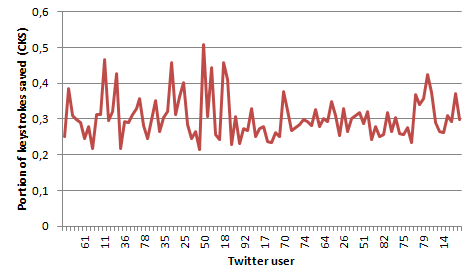
\includegraphics[scale=1.0]{twitter_chaos}
\caption{The proportion of keystrokes saved for individual Twitter users, ordered by number of tweets (from left to right: from least to most), when using the best-performing module set-up}
\label{chaos}
\end{figure} 


The large amount of variation between individual Twitter users cannot easily be explained, with a few exceptions (for example, people with powerful idiolect models sometimes often repeated long words like \emph{goedemorgen} 'good morning', \emph{dankjewel} 'thank you', and \emph{welterusten} 'sleep well'), but no clear patterns emerged. Trying to predict for which persons word prediction will go well and for which persons it will not might be an interesting topic for future research. It is a question that is related to the field of computational stylometry and in particular automatic authorship attribution, although authorship attribution is the exact opposite of the task described here (guessing the author on the basis of text instead of guessing the text on the basis of the author) \cite{bagavandas+08}.

\begin{table*}[htb] 
\centering
\begin{tabular}{ll|llll} 
Training material&Test material&\multicolumn{2}{l}{CKS}&\multicolumn{2}{l}{SKKS}\\
\hline
&&Mean&St. dev.&Mean&St. dev.\\
Idiolect&Twitter feed&29.6&6.4&32.1&6.3\\
Control model&Twitter feed&31.2&6.3&33.9&6\\
Sociolect&Twitter feed&33.9&7.1&36.2&7.1\\
\end{tabular} 
\caption{Mean percentage of keystrokes saved when using an idiolect, a control model (consisting of an idiolect and random other Twitter feeds) and a sociolect.} \label{socio_results}
\end{table*}

\begin{table*}[htb] 
\centering
\begin{tabular}{l|llllll} 
Twitter user&\multicolumn{2}{l}{Idiolect}&\multicolumn{2}{l}{Idiolect+random feeds}&\multicolumn{2}{l}{Sociolect}\\
\hline
&CKS&SKKS&CKS&SKKS&CKS&SKKS\\
24&31.2&36.3&34&36.4&31.6&34.3\\
49&27.2&29.1&26.2&29.7&24.6&27.2\\
71&27.5&30.2&34.2&35.8&30.8&32.9\\
\end{tabular} 
\caption{Percentage of keystrokes saved for 3 atypical Twitter users, using the the idiolect, control and sociolect models}
\label{deviations}
\end{table*}

\subsection{Social networks and language input} \label{input_networks}

The findings by Lesher {\em et al.} \citeyear{Lesher+99} suggest that more material leads to more keystrokes saved; this may also hold for idiolects. This material, however, might not be available, simply because not all people write or tweet that much. For a particular user $x$, what other sources of language do we have that might be similar to the idiolect of $x$? One of the more obvious answers might be the language of the people $x$ often communicates with. The fact that people that are in some way related to each other speak alike using a 'group language' or a sociolect, is well established in sociolinguistics.

This approach of including the language of the people from a particular person's environment can also be viewed from a different perspective: so far, we have followed Mollin \citeyear{mollin09} and Barlow\citeyear{barlow10} in using only the \emph{output} of speakers. This makes sense (since what comes out must have been inside), but can never be the full story. The sociolect model that will be constructed here can be seen as a feasible and rough approximation of recording everything a person reads or hears: by including the language of the socially related persons of person $x$, the system can have a rough idea of the kind of \emph{input} person $x$ gets.

On the basis of the data already collected for the idiolect experiments, sociolects were created by collecting all addressees mentioned with the \emph{@addressee} syntax for each of the 100 Twitter users used in the previous experiment. For all addressees that were mentioned three times or more, it was checked if this addressee was in the dataset (which was almost always the case). If so, it was checked whether this addressee also mentioned the original Twitter user at least three times. If this was also the case, the system assumed the users speak to each other often enough to have their language adjusted to each other, and the tweets of this addressee were added to the sociolect of the original Twitter user. We thus end up with 100 sociolects built around the 100 most active Twitter users, all based on the tweets of a Twitter user and the tweets of the persons that this person communicated with at least six times (three times as writer, three times as reader).

The results of Verberne {\em et al.} \citeyear{verberne+12} would predict that adding tweets in general would lead to increases in the number of keystrokes saved, as this is using more texts from the same genre. To be sure that any improvements can be attributed to the fact that this is the language from friends, a control model will be built. While the sociolect model consists of the tweets of Twitter user $x$ and the tweets of the friends of twitter user $x$, the control model consists of the tweets of Twitter user $x$ and the tweets of random other Twitter users, and has approximately the same number of words.

For each of the 100 Twitter users, comparative runs are performed with the model created on the basis of the idiolect and the random Twitter users versus the sociolect model. The best performing module set-up from the previous experiments is used.  The results are compared to the simulations with the idiolect model from the previous experiment. The results of the simulations are summarized in Table \ref{socio_results}.
We observe that adding more tweets to the idiolects leads to more keystrokes saved, and that the most keystrokes can be saved when using the tweets of the people the owner of the idiolect communicates with often.

An ANOVA for repeated measures showed that there is a significant effect for the training material $F(2,198) = 69.466, p < .001$. Contrast analyses revealed that both the differences between the results of the idiolect model and the idiolect model and random feeds $F(1,99) = 93.471, p < .001$ and the idiolect model and random feeds and the sociolect model $F(1,99) = 61.871, p < .001$ are significant.

Again, the high standard deviations indicate notable variation among the individual results. Table~\ref{deviations} lists the deviating individual scores for three individual Twitter users. In these results we see an increase when random tweets are added, but a decrease when the tweets from their conversation partners are used. For user 24 and 49, the percentage of keystrokes saved when using the sociolect model is even lower than the idiolect model alone.  

Using the best-performing module set-up in general, the set-up with the sociolect model, backed up by the general language model, \emph{and} the recency buffer, the worst result is 21.3\% CKS and 22\% SKKS for user 90, and the best result is 56.2\% CKS and 58.1\% SKKS for user 38.


\section{Conclusion} \label{conclusion}

In this paper we presented the word prediction system \emph{Soothsayer}. Testing the system we found that word prediction and idiolects are an effective combination; our results show that word prediction is best done with a combination of an idiolect-based context-sensitive system, backed up by a context-sensitive module equipped with a general language model. A recency buffer is a useful third module in the sequence. Our average best scores with these three modules are 29.7\% keystrokes saved according to the strict (one-best) CKS metric, and 32.1\% keystrokes saved according to the Swiftkey-inspired SKKS metric. 

The fact that people speak like the people around them can also be useful to word prediction. When we approximate a sociolect by expanding a user's Twitter corpus by tweets from people this person communicates with, and retrain our first context-sensitive module with this data, average scores improve to 33.9\% CKS and 36.2\% SKKS.

What works well for one speaker, might not necessarily work for another, however. While we find significant advantages of idiolect-based and sociolect-based training, the variation among our 100 test users is substantial, and in individual cases idiolect-based training is not the best option. For other users the positive gains are substantially higher than the mean; the best result for a single user is 56.2\% CKS and 58.1\% SKKS.

In future research we aim to investigate methods that could predetermine which model and module order will work best for a user. 
Another set of open research questions concern the fact that we have not tested many of the system's settings. What would be the effects of predicting more words at the same time?

%\section{Acknowledgements/dankwoord}

\bibliography{thesisbib}{}
\bibliographystyle{apacite}

\end{document}
